%Written by: Aaron Stillmaker
%October 23, 2018
%ECE 186A - Senior Design
%
%This is a template you can use for your Project Charter, though you will need to change a good portion of it for your own needs.

\documentclass[12pt,onecolumn]{IEEEtran}			%Everything is default, except  which is journal, 10pt font, and final draft

%add packages here:
\usepackage{comment}
\usepackage{vhistory}
\usepackage[utf8]{inputenc}
\usepackage{graphicx}
\usepackage{caption}
\usepackage{pdfpages}
\usepackage{placeins}
\usepackage{chngcntr}


\graphicspath{ {figures/} }

\title{ \hfill  \vspace{2in} \\ Drone Position and Navigation using Machine Vision  \vspace{1in} }	%the \vspace is moving the title down from the top of the page
\author{California State University, Fresno \\
Electrical and Computer Engineering Department \\
ECE 186A - Senior Design I \\ 					%I am jamming all of the stuff I want on the title page into the Author spot, I know, this isn't elegant
Spring 2021 - Dr. Stillmaker \\ 					%Note the \\ line returns to make sure to put each one on a new line

\vspace{12pt} 								%I put in some space to get the due date listed a little lower
By: Alexander Her 
\&
Gilbert Barr \\
Co-Technical Advisor - Dr. Hovannes Kulhandjin \\
Co-Technical Advisor - Dr. Hayssam El-Razouk
\vspace{2in}								%You may need to mess with this space, this space is above the signature lines.


\vspace{4in}}								%You will need to mess with this space, this space is after the signature lines.  The idea
										%is to make the title page by itself.  I know, this isn't elegant either, but IEEE formatting doesn't
										%make title pages

\begin{document}


\maketitle									%This generates the title from the information given above.
\thispagestyle{empty}						%This removes the page number from the title page.
\newpage

\newpage


 


\begin{versionhistory}
  \vhEntry{1.0}{03.08.21}{AH|GB}{ This revision is the first version of the project description. This document was written by both Alexander and Gilbert. They finalized the document on March 8, 2021 and the changes that were made included: Introduction, Abstract, Project Objectives and Success Criteria, High-Level Requirements, Assumptions, Constraints, and Standards, and Project Description and Boundaries. }
  \vhEntry{1.1}{04.05.21}{AH|GB}{Adjusted document to clarify objective of project, updated revision table, and add new advisor }
  
\end{versionhistory}


\newpage 
\tableofcontents % for the future make sure to add list of figures and tables. 

\newpage
\listoffigures
\listoftables



 
 \newpage 
 \section*{Abstract}
 This project is the implementation of a computer vision algorithm that is able to accurately detect and provide positional data of a small drone in an indoor environment. It will be very useful in applications such as aerial deliveries, rescue operations, and warehouse logistics.The project will consist of a base station with a mounted camera that is pointed down towards the base station. The camera will be connected to a small embedded computer capable of running our algorithm and communicating with our drone. 
 
 The algorithm will be implemented using a convolutional neural network as these are the best type of networks for processing image data. Our network will be built using the Pytorch framework which will provide us with the building blocks and flexibility to create our own network quickly.
 
 On the controls side of the project they will be utilizing a drone that allows for complete control directly from a computer interface as opposed to a conventional radio system that uses a handheld remote. For this section of the project code must be developed that can take positional data from a neural network and relay the appropriate movement commands to our drone.
 
 
 \section{Introduction}
The project will focus on utilizing machine learning to detect and provide positional data of a small drone using machine vision. In this project machine learning will be utilized to infer the the position of a drone which will allow for control and navigation in a limited area [1]. It will be necessary to implement an interface between the machine learning algorithm and the communication system of the drone. \\

\begin{figure}[hp]
    \centering
    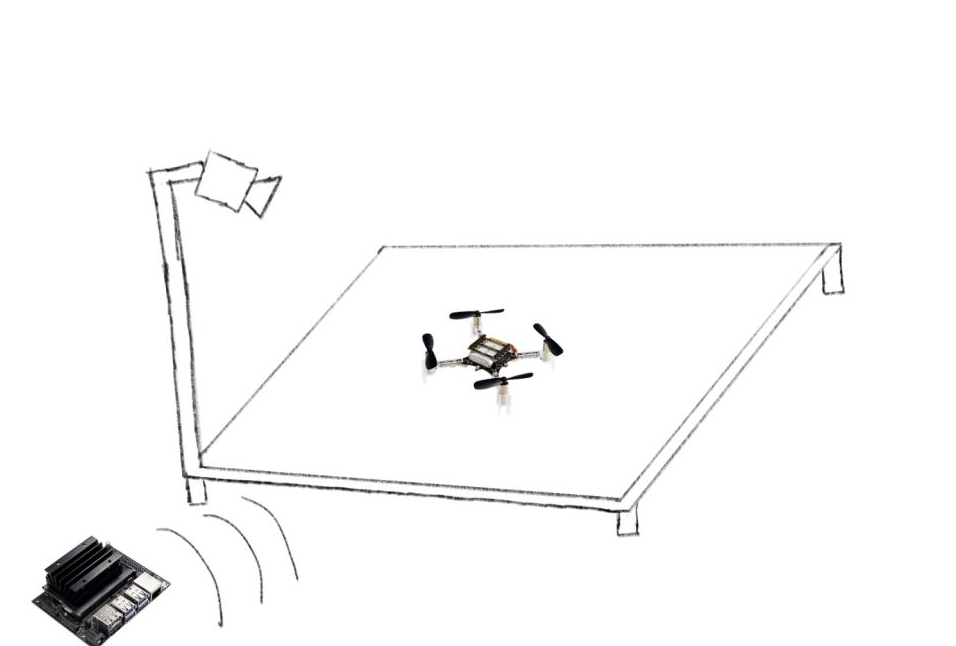
\includegraphics[width=12cm]{Images/senior design figure.PNG} 
    \caption{Base Station with Drone, Jetson NANO, OpenCV, and Oak-D Camera}
    \label{fig:project_overview}
\end{figure}


\section{Required Background Knowledge}
The knowledge that will be most required for the completion of this project will be software related. This is due to the fact that the algorithms that will be developed will be done so over in software. The algorithms will be developed in Python and will utilize the Pytorch framework library. Pytorch is a machine learning library that will allow the group to develop the model. This model will be developed using Transfer Learning which utilizes a pre-existing model that solves one problem to be developed to solve a different but related problem. It will also be important that there is a good understand of how Machine Learning works because the project's main problems will be based heavily on how efficiently the algorithms are written. 

\vspace{12pt} 


\textbf{Alexander Her} (Project Manager)\\ 
\textbf{Major:} Computer Engineering\\
\textbf{Responsibilities:} Alexander is responsible for developing the machine learning algorithms using Pytorch or Tensorflow. \\

\textbf{Gilbert Barr}\\
\textbf{Major:} Computer Engineering\\ 
\textbf{Responsibilities:} Gilbert is responsible for the computer controls system of the drone as well as data set collection. \\ 



 
 \section{Project Objectives and Success Criteria}
 
 \vspace{12pt} 
 
  \begin{figure}[hp]
    \centering
    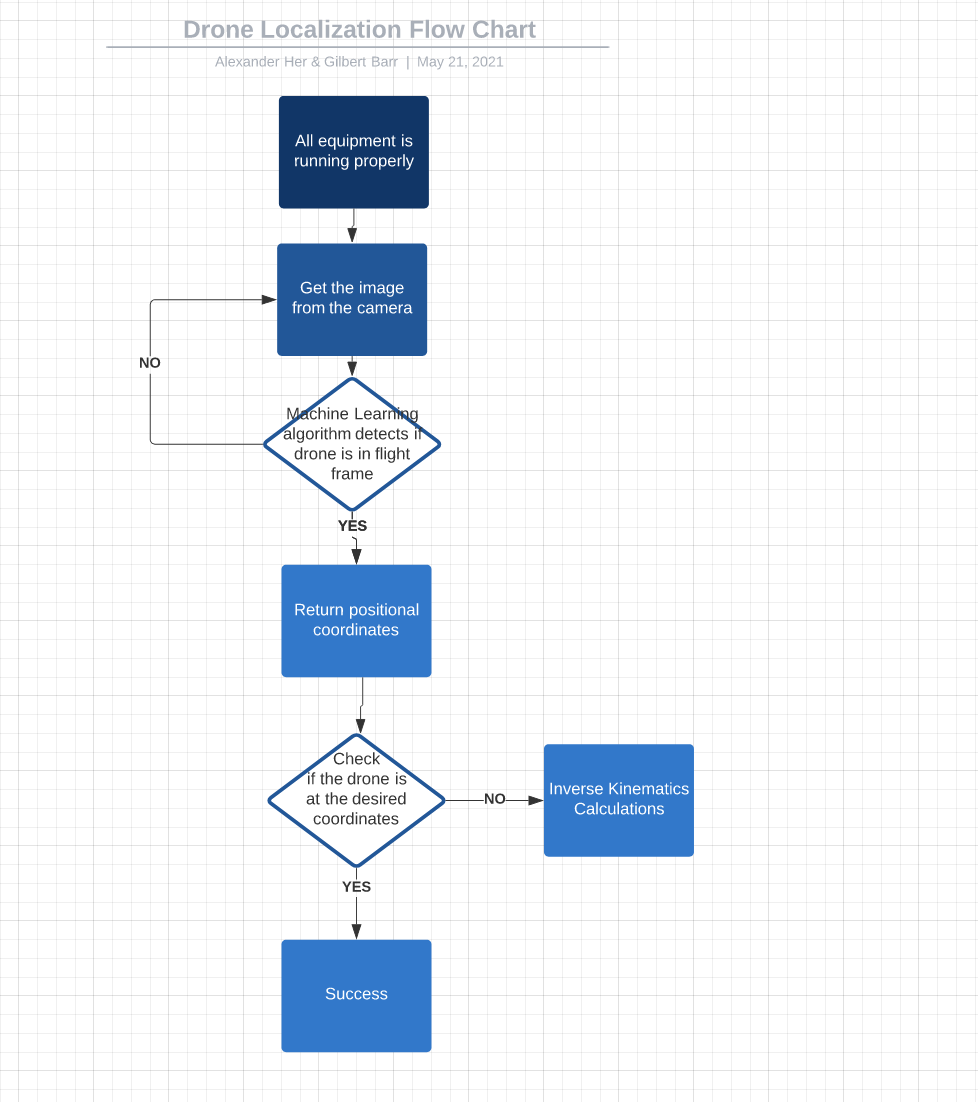
\includegraphics[width=12cm]{Images/drone localization flow chart.PNG} 
    \caption{Drone Localization Flow Chart Overview}
    \label{fig:Drone Flowchart}
\end{figure}

 
 \textbf{Main Project Objectives:}

The project objective to utilize machine vision algorithms for drone localization, detection, and control a small indoor drone. For the scope of this project, we will be using transfer learning to speed up the development and training of a model that can detect our drone in a small, enclosed environment. Once we have an algorithm that can accurately detect the position of the drone in real time, we will use it to maneuver to set positions within our enclosed environment. For this project, a base station consisting of an embedded computing platform will be used with a camera to perform the machine learning computations as well as communicate and maneuver the drone.
  




\vspace{12pt} 

 \textbf{Success Criteria:}

 \begin{description}
  \item[$\bullet$ ] To have the machine vision algorithm developed enough to accurately detect drone position within 5cm error. 
  \item[$\bullet$ ] To set up a target route for the drone in the airspace and have it maneuver without issues. 
  \item[$\bullet$ ] To be able to detect objects in the environment and avoids any collisions. 
\end{description} 
\vspace{12pt} 


 
 \section{High-Level Requirements}

 
\textbf{Basic Requirements:}

 \begin{description}
  \item[$\bullet$ ] The project should be implemented in 2 semesters. 
  \item[$\bullet$ ] The project shall be completed given the budget that was proposed. 
  \item[$\bullet$ ] The project shall be tested extensively along project development. 
  
\end{description} 

\vspace{12pt} 

 \textbf{Milestone Tasks:}
 
 \begin{description}
  \item[$\bullet$ ] Access to the Unmanned System Research Team (USRT) lab will be crucial to the development of this project due to the tools that are offered in the laboratory. 
  \item[$\bullet$ ] Proper design of the quad-copter frame will ensure that the drone can go through intensive testing.  
  \item[$\bullet$ ] Efficient machine learning algorithms that will allow for the quad-copter drone to effectively maneuver through the indoor airspace. 
\end{description} 

\vspace{12pt} 

\textbf{Hardware Requirements:}
 
 \begin{description}
  \item[$\bullet$ ] The drone, through the use of a base station, should be able to utilize the machine learning algorithm for making movements accordingly. 
  \item[$\bullet$ ] The embedded computer should be able to utilize external hardware such as a camera. 
  \item[$\bullet$ ] The embedded computer should be able to get positional data from the camera utilizing the neural network. 
\end{description} 

\vspace{12pt} 

 \textbf{Software Requirements:}
 
 \begin{description}
  \item[$\bullet$ ] The machine learning algorithm should be implemented using Pytorch or Tensorflow. 
  \item[$\bullet$ ] The algorithm should be implemented using a convolutional neural network for processing image data. 
  \item[$\bullet$ ] The machine learning algorithm should be able to give the drone the correct coordinates for maneuvering in the airspace.
\end{description}
\vspace{12pt} 


\section{Test Plan}
\begin{table}[h!]
\begin{center}
\begin{tabular}{| m{3cm} | m{13cm}| } 
 \hline
  OpenCV AI Kit: Oak-D Camera & The success criteria for the camera tests will be that the camera must be able to send photos to the Jetson NANO and it must be able to send multiple photos. Gilbert Barr will be in charge of making sure that this works. The tests will be stopped if the images are not able to be uploaded to the Jetson NANO.   \\
 \hline
 Crazyfile 2.1 & The success criteria for the drone will be if the Jetson NANO will be able to send movement commands to the drone and if the movement error is within ±5 inches of input from the Jetson NANO. These tests will be run by Gilbert Barr. The tests will be stopped if the drone cannot fly properly and safely.   \\
 \hline
 Jetson NANO & The success criteria for the Jetson NANO will be if the device will be abble to take in images and detect the drone in the base station airspace. The images should also be able to detect the drone within ±5 seconds of input from the depth sensing camera. These test will be run by both Gilbert Barr and Alexander Her. The tests will be stopped if the Jetson NANO cannot run the Machine Learning algorithm in real time.   \\
 \hline
 Data Set Collection & The success criteria of the data set collections will be if ther camera will be able to detect the drone in the picture frame. The distance from label to drone should also be within ±3 cm. These tests will be run by both Gilbert Barr and Alexander Her. The tests will be stopped if the group is not able to properly label the images that will be collected.    \\
 \hline
 Machine Learning Algorithm & The success criteria of the algorithm will be if the algorithm is able to detect the drone in the picture frame and if the accuracy is higher than 90\&. The tests will be run by Alexander Her since his responsibility will be developing the algorithm. The tests will be stopped if the algorithm is not able to run real time on the Jetson NANO and accurately detect the drone within the picture frame.  \\
 \hline
\end{tabular}
\end{center}
\caption{Test Plans}
\label{Test Table:1}
\end{table}

 
\section{Assumptions, Constraints, and Standards}
Alexander and Gilbert are both Computer Engineering majors and have taken similar classes. Alexander has experience working with software development while Gilbert has experience working with control systems and robotics. Alexander is unfamiliar with robotics and has to learn a lot of keep up with Gilbert's extensive knowledge about drones. Both of the students are unfamiliar with machine learning and plan to learn together throughout the two semesters that they are given. 
The background information that will be needed to complete the project would be knowledge about machine learning as well as any additional information about the hardware that they want to utilize. Some courses that will be helpful in completing this project will be: 

 \begin{description}
  \item[$\bullet$ ] ECE 71, 81, 141, 155, 172, 173
  \item[$\bullet$ ] CSCI 40, 41
\end{description}
\vspace{12pt} 

\underline{ECE 71 / CSCI 40}
\vspace{6pt} 

ECE 71 and CSCI 40 are both introduction courses to programming and will need to have been a prerequisite for this project because this project will utilize Python which is a Object-Oriented language. In these courses, students are first introduced to Object-Oriented programming.

\vspace{6pt}

\underline{ECE 81 / CSCI 41}
\vspace{6pt}

ECE 81 and CSCI 41 are the courses that would usually be taken after ECE 71 pr CSCI 40. These two courses focus on learning how data structures and algorithms work. These concepts will be very important in our project since we will be developing an algorithm to maneuver our drone. 
\vspace{6pt} 

\underline{ECE 141}
\vspace{6pt} 

ECE 141 will be an important course because this course, Algorithmic Computations, is a continuation of the introduction to Data Structures and Algorithms course. This course will be very useful in developing an efficient and complex algorithm. 

\vspace{6pt} 
\underline{ECE 155}
\vspace{6pt} 

ECE 155, Controls Systems, covers topics including PID controllers and how to tune them. For the custom drone, minor modifications and tuning to the PID coefficients will be necessary so basic knowledge on PIDs is necessary.

\vspace{6pt} 
\underline{ECE 172}
\vspace{6pt} 

ECE 172, Machine learning, covers topic such as machine vision and different image processing models and algorithms.

\vspace{6pt} 
\underline{ECE 173}
\vspace{6pt} 
 
ECE 173, Robotics, covers robotic control theory topics such as kinematics and inverse kinematics. Inverse kinematics will be used to calculate the drone movements necessary to maneuver from its position to a desired position.
 
\section{Project Description and Boundaries}

The project implementation was already explained in earlier sections so this description will serve as to provide the purpose of the project. The team's goal and vision of the completed project will be that it can be utilized in workplaces such as warehouses so that moving items could be a lot easier when vertical maneuverability is needed. The team believes that if they could develop an efficient machine learning algorithm then this could be very helpful for any packaging company in the industry. 

Some potential difficulties of this project will be developing a machine learning algorithm since this is a field that both the students are not too familiar with. They will also need to learn how to use python frameworks such as Pytorch and Tensorflow that utilize machine learning models. Once that obstacle is overcome, the next main issue would be interfacing the algorithm with the drone to make sure that it is working effectively. They believe that most of the work done in this project though will be done developing the machine learning algorithm by making it as effective as possible. 

One of the technical advisors that would be a great fit for this project will be Dr. Kulhandian because his extensive knowledge of Machine Learning will be very helpful in the completion of this project. He will be the best advisor for this project since we are focusing primarily on Machine Learning.

Another technical advisor that would be a great fit for this project would be Dr. El-Razouk since he is currently teaching the algorithms courses in the ECE department. His knowledge in algorithms will be very helpful when the Machine Learning algorithms are being developed. 



\section{High-Level Risks}
Since the drone will be tested a lot and could pose a potential risk if it happens to go out of control. This should be the only risk that the team should be worried about. How this will be handled will be through: 
\vspace{12pt} 
 \begin{description}
  \item[$\bullet$ ] Keeping at a safe distance when testing so that no injuries are at risk. 
  \item[$\bullet$ ] Incremental testing that allows for testing each feature. 
  \item[$\bullet$ ] Checking quality of hardware constantly by performing quality checks before flight runs. 
\end{description}



\section{Equipment and Budget}
The team should have most of the equipment that is needed for this project. For extras, an extra camera could be purchased so that the team could further develop their algorithm if it is successful. 
\vspace{12pt} 

Current Equipment in Inventory:

\begin{table}[h!]
\begin{center}
\begin{tabular}{| m{3cm} | m{13cm}| m{1cm} |} 
 \hline
  Item & Reason  & Price \\
 \hline
 OpenCV AI Kit: Oak-D Camera & Stereo Camera developed to work with OpenCV  & \$100 \\
 \hline
 Jetson Nano & The embedded computing platform that will be utilized for machine learning inference and drone control  & \$100 \\
 \hline
 Crazyflie 2.0 & Small drone used for proof of concept and testing interface with Jetson Nano & \$195 \\
 \hline
 Crazyflie Bolt & The Bolt is the new platform that will be utilized for it flexibility and customizability. This will be the flight controller for our custom done platform that must be designed from scratch and built & \$200 \\
 \hline
 Crazyflie Add-on: Flow Deck & T & \$50 \\
 \hline
 Crazyflie Add-on: Multi-Ranger Deck & T & \$80 \\
 \hline
 Crazyflie Add-on: Lighthouse Deck & T & \$80 \\
 \hline
 Two SteamVR Base Station 2.0 & T & \$300 \\
 \hline
\end{tabular}
\end{center}
\caption{Budget Plans}
\label{Inventory Table:2}
\end{table}

 \begin{description}
  \item[$\bullet$ ] OpenCV AI Kit: Oak-D Camera
  \item[$\bullet$ ] Jetson NANO
  \item[$\bullet$ ] Crazyfile 2.0 Quad-Copter
  \item[$\bullet$ ] Two SteamVR base station 2.0
\end{description}

\vspace{12pt} 

Funds request:

 \begin{table}[h!]
\begin{center}
\begin{tabular}{| m{3cm} | m{13cm}| m{1cm} |} 
 \hline
  Item & Reason  & Price \\
 \hline
 OpenCV AI Kit: Oak-D Camera & Another camera is being requested because the plan of the project is to hopefully be able to utilize multiple camera angels and with the addition of this camera, that will be possible.  & \$100 \\
 \hline
 PVC Pipes for constructing camera mount & To construct the camera mount, the best material that was thought of to ensure stable captures of the base station was PVC Pipes. & \$50 \\
 \hline
 Crazyflie 2.1 & An additional drone so both students can do development and testing would be beneficial. & \$225 \\
 \hline
\end{tabular}
\end{center}
\caption{Budget Plans}
\label{Budget Table:2}
\end{table}
\vspace{12pt} 
 
 
 \section{Approvals}
\vspace{12pt} 
\vspace{12pt} 



\begin{tabular}{@{}p{.5in}p{4in}@{}}
Approved: & \hrulefill \\
& Alexander Her \\
& Computer Engineering\\
\end{tabular}
\vspace{12pt} 

\begin{tabular}{@{}p{.5in}p{4in}@{}}
Approved: & \hrulefill \\
& Gilbert Barr \\
& Computer Engineering\\
\end{tabular}
\vspace{12pt} 

\begin{tabular}{@{}p{.5in}p{4in}@{}}
Approved: & \hrulefill \\
& Hovannes Kulhandjian, Ph.D \\
& Assistant Professor\\
\end{tabular}
\vspace{12pt} 

\begin{tabular}{@{}p{.5in}p{4in}@{}}
Approved: & \hrulefill \\
& Hayssam El-Razouk, Ph.D \\
& Assistant Professor\\
\end{tabular}


\newpage
~\cite{lu2018survey}
~\cite{mishra2019introduction}
~\cite{shanmugamani2018deep}
\bibliographystyle{plain}
\bibliography{biblography.bib}
 

\end{document}


